\documentclass[11pt]{article}
\usepackage[top=.6in, bottom=.6in]{geometry}
\usepackage{graphicx, float, tikz}
\usepackage{amsmath, amssymb, amsthm}
\def\doubleunderline#1{\underline{\underline{#1}}}
\usepackage{enumerate}
\usepackage{color, soul}
\usepackage[normalem]{ulem}
\usepackage{hyperref}

\begin{document}
\title{\Large CS 4331-002: Special Topics in CS - Virtual Reality \\ Spring 2018 Student's Choice Presentation: Report \\ \Large Simon Woldemichael \\ Tuesday, February 6, 2018 \\}
\author{\LARGE \textbf{NVIDIA Holodeck}}
\vspace{-2cm}
\date{}

\maketitle
\vspace{-1cm}
\hspace{30pt}

\begin{center}
\textbf{Abstract}\\

NVIDIA Corporation's Project Holodeck is a high-end, photorealistic virtual reality environment designed for collaborative prototyping and design. The interface was developed to become an industrial standard. Although it is less than a year old, has higher than average hardware requirements, and has not been fully released, it is already being used by several commercial companies and firms within today's industry.
\end{center}
\centerline{
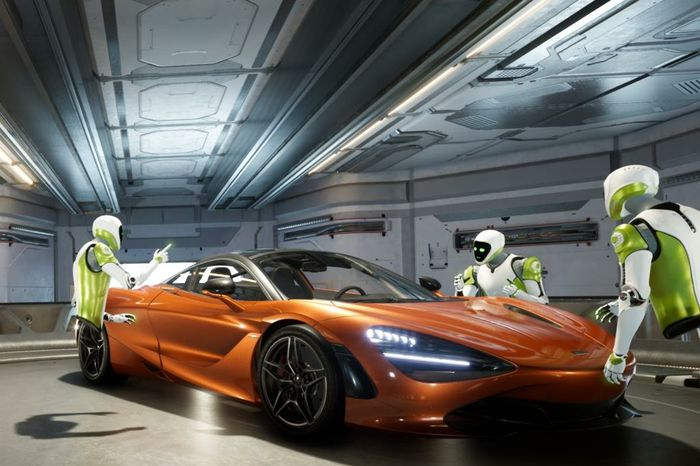
\includegraphics[scale=.4]{../images/Holodeck-web.jpg}}
\paragraph{Overview} ~ \par 
Currently in an Early Access phase and announced at last years GPU Technology Conference (GTC), NVIDIA Holodeck, also aliased as Project Holodeck, is NVIDIA Corporation's innovative idea at speeding up and improving the creativity process \cite{nvidianews}. The platform, utilizing NVIDIA's own middle to high-end GPUs, was developed for designers, peers, and stakeholders to collaborate in a more 3D, virtual environment \cite{nvidiamain} with a high degree of freedom and flexibility. The environment involves the loading of fully developed and highly intricate Computer Aided Design (CAD) models, made with AutoDesk Max or AutoDesk Maya. With the help of the Holodeck, these high-detail, highly precise models give designers all of the information they need to go from prototype to final product. While there have been attempts at designing a \emph{Holodeck}, attributed to an environment with the same name and features as that of \emph{Star Trek}'s Holodeck, none have been able to reach a capacity comparable to that of NVIDIA's implementation.

\paragraph{Where is it used?} ~ \par 
Currently, the VR environment is publicly used by 3 companies who were approved for Early Access \cite{nvidiamain}; \textit{Koenigsegg Automotive AB}, \textit{NASA}, and \textit{Kohn Pedersen Fox}. Additionally, Project Holodeck is being used by NVIDIA to strengthen AI-based robot training. \par
Koenigsegg uses the Holodeck for collaborative automotive design. The CAD model for their $1.9$M USD Regera supercar contains over $50,000,000$ polygons, all of which can be loaded quickly into the Holodeck. Instead of having to compress the model for distribution, loading, and viewing, the model can be presented into the Holodeck directly from its CAD file \cite{nvidiamain}. The \textit{clipping sphere} and \textit{explode} tools packaged with the Holodeck can then be used to view every single part of the car for another layer of detailed, high-fidelity inspection and design \cite{nvidiablog3}.  \par
NASA uses the Holodeck to simulate the effects that extra-terrestrial dynamics have on rover and probe designs \cite{nvidiamain}. Additionally, the Holodeck assists scientists and engineers create the actual models that will be used for testing the efficiency and safety of those designs.  \par
Architecture firm Kohn Pedersen Fox uses the Holodeck for accurate visual and physical prototyping.  Kohn Pedersen Fox's Senior Associate Principal and Applied Research Director, Cobus Bothma says, ``NVIDIA Holodeck is going to enable us to deliver on this potential, with amazingly accurate visuals and physics. And, it will allow us to collaborate with designers in our worldwide offices, our partners, and our clients, in real-time. That’s a powerful game changer for our industry'' \cite{nvidiamain}. \par
Lastly, in last years Association for Computing Machinery Special Interest Group on Computer Graphics and Interactive Techniques (ACMSIGGRAPH) conference, NVIDIA immersed its robot ``NVIDIA Isaac'' in the Holodeck. Backed by deep learning, computer vision and 2 neural networks, Isaac interacted with SIGGRAPH guests to sharpen and develop more life-like and realistic actions \cite{nvidiablog3} all through the medium of a game of dominoes within the Holodeck. 
	
\paragraph{How does it work?} ~ \par 
Taking into consideration that the Holodeck has not been made fully available to the public, is closed-source, a sophisticated piece of commercial software, and its young age, it is not unreasonable that its exact inner workings are unknown. According to the initial news post released by NVIDIA shortly after GTC 2017, \cite{nvidiablog1} Project Holodeck is built on an enhanced version of software and video game development company Epic Games' Unreal Engine 4 and, ``includes NVIDIA GameWorks, VRWorks and DesignWorks delivering unparallel photorealism and physics simulation in collaborative virtual reality.'' The latter 3 are all licensed middleware software suites used by a majority of high graphics computation hardware (i.e. video game consoles and GPUs) to process physics, lighting, special effects, realistic virtual reality, and all other tasks that require large amounts of graphical computation.

\paragraph{Why is this a good use of virtual reality?} ~ \par 
Firstly, the Holodeck is not bound to local interation. This means, collaborators from anywhere in the world can join the same Holodeck environemnt, given they have the hardware requirements and permissions to join the host. Instead of having to transport a car or incomplete building many miles away so that current designers and other contributors may be in the same space to work on a prototype or precursor to a large project, the model simply has to be loaded into the Holodeck and all collaborators can work on the same model, in real-time and high fidelity. 

Secondly, the Holodeck is an not a finite space. The amount of space that you can simulate in a virtual world is only bound by your own computational capabilities. For example, instead of a municipal authority spending millions of dollars to build a school, it would be ideal, hypothetically, to spend a single hundred thousand dollars on a supply of high-end GPUs, NVIDIA's 1,200 USD Titan Xp for example. A municipal authority can then form a cluster from these GPUs to run a live Holodeck that would house a classroom. Students, along with a single or multiple instructors, from all over the world would then be able to connect to this Holodeck to learn content no different from that which would be present in a live, traditional classroom. This methodology could \emph{definitively and effectively} eliminate the need for a central educational authority (i.e. college or university) and would drastically cut the cost of going to school. College campuses would be replaced with top-of-the-line computational powerhouses full of thousands of virtual students.

\paragraph{User experience} ~ \par  
Once again, since Project Holodeck is relatively new compared to many of the other virtual reality technologies present, and because its hardware requirements are very high-end and expensive compared to what most people have access to, there have not been many end-user interactions with the product. But, from demonstrations given by NVIDIA at several conferences \cite{video1, video3} the framework does not seem to cause any varying degrees of nausea, fatigue, headaches, eyestrain, vertigo or dizziness. While I have not personally tried the Holodeck, from the demonstrations and examples \cite{video1}, one of which was live during GTC \cite{video4}, I would rank Project Holodeck a \textbf{0} on its chances of giving users any degree of simulator sickness.

\paragraph{Getting Involved} ~ \par
Despite Project Holodeck's age, NVIDIA is greatly pulling for users to try the platform for themselves \cite{nvidiablog2}. \emph{Anyone} who meets system requirements can apply for Early Access at \url{www.nvidia.com/holodeck}. The requirements for effectively running an instance of the Holodeck include the following:
\begin{center}
\begin{enumerate}
\item[$\bullet$]GPU: Quadro P6000, Geforce GTX 1080Ti, or TITAN Xp
\item[$\bullet$]VR Headset: HTC Vive or Oculus Rift with Touch controllers
\item[$\bullet$]CPU: Intel Core i7-6700K or greater
\item[$\bullet$]Memory: 16GB RAM
\item[$\bullet$]Hard drive: A SSD or fast HDD
\item[$\bullet$]Operating System: Windows 10 Service Pack 1 (64-bit)
\item[$\bullet$]Access to a Steam account
\end{enumerate}
\end{center}

\paragraph{Conclusion} ~ \par 
When the Holodeck is released officially, I believe there will be much more to talk about in regards to strengths, weaknesses, applications and limitations. At it's current state, Project Holodeck is an amazing innovation that is definitely effective in delivering on the specifications of its indented use. I predict, as technology develops and GPUs become increasingly powerful, Project Holodeck will be used all over the world.

% Begin bibliography page
\newpage
\begin{thebibliography}{10}
\bibitem{nvidiamain} 
\textit{Design \& Professional Visusalization Solutions}. NVIDIA, \url{www.nvidia.com/en-us/design-visualization/technologies/holodeck/}.
 \bibitem{nvidiablog1} 
\textit{NVIDIA Reveals Holodeck, Its Groundbreaking Project for Photorealistic, Collaborative VR.} 
The Official NVIDIA Blog 10 Aug. 2017, \url{www.blogs.nvidia.com/blog/2017/05/10/holodeck/}.
\bibitem{nvidiablog2} 
\textit{Join Us as We Build NVIDIA Holodeck.} The Official NVIDIA Blog, 13 Nov. 2017, \url{www.blogs.nvidia.com/blog/2017/10/10/holodeck-design-lab-of-the-future/}.
\bibitem{nvidianews} 
\textit{Welcome to the Holodeck, NVIDIA's Design Lab of the Future}. NVIDIA Newsroom, \url{http://nvidianews.nvidia.com/news/welcome-to-the-holodeck-nvidia-s-design-lab-of-the-future}.
\bibitem{techcrunch} 
Etherington, Darrell. \textit{Nvidia built a real Holodeck, aimed at creative collaboration.} TechCrunch, 10 Oct. 2017, \url{www.techcrunch.com/2017/10/10/nvidia-built-a-real-holodeck-aimed-at-creative-collaboration/}.
\bibitem{nvidiablog3}
\textit{Dominoes Anyone? SIGGRAPH Attendees Go Head-to-Head with Isaac-Trained Robot in VR and Real Life.} The Official NVIDIA Blog, 24 Oct. 2017, \url{www.blogs.nvidia.com/blog/2017/07/31/dominoes-siggraph-isaac-vr-ai/#source=pr}.
%Video sources
\bibitem{video1}
ddayvideo. \textit{NVIDIA Holodeck, the demo}, YouTube, DDay.it, 13 Oct. 2017, \url{www.youtube.com/watch?v=DLCS0U7B0gY}.
\bibitem{video2}
NVIDIA. \textit{NVIDIA Holodeck: Photorealistic Collaborative Design in VR}, YouTube, 13 Nov. 2017, \url{https://www.youtube.com/watch?v=goFZOTjCVFg}
\bibitem{video3}
Digital Trends. \textit{Collaborate in Virtual Reality with Nvidia's Holodeck - CES 2018}, Youtube, 11 Jan. 2018, \url{https://www.youtube.com/watch?v=bFNI3IJi0_c}
\bibitem{video4}
NVIDIA \textit{GTC Japan 2017 Part 3: New NVIDIA Holodeck with Lexus}, Youtube, 15 Dec. 2018, \url{https://www.youtube.com/watch?v=0e4187XNaW4}

\end{thebibliography}
\end{document}